\documentclass[twoside]{book}

% Packages required by doxygen
\usepackage{fixltx2e}
\usepackage{calc}
\usepackage{doxygen}
\usepackage[export]{adjustbox} % also loads graphicx
\usepackage{graphicx}
\usepackage[utf8]{inputenc}
\usepackage{makeidx}
\usepackage{multicol}
\usepackage{multirow}
\PassOptionsToPackage{warn}{textcomp}
\usepackage{textcomp}
\usepackage[nointegrals]{wasysym}
\usepackage[table]{xcolor}

% Font selection
\usepackage[T1]{fontenc}
\usepackage[scaled=.90]{helvet}
\usepackage{courier}
\usepackage{amssymb}
\usepackage{sectsty}
\renewcommand{\familydefault}{\sfdefault}
\allsectionsfont{%
  \fontseries{bc}\selectfont%
  \color{darkgray}%
}
\renewcommand{\DoxyLabelFont}{%
  \fontseries{bc}\selectfont%
  \color{darkgray}%
}
\newcommand{\+}{\discretionary{\mbox{\scriptsize$\hookleftarrow$}}{}{}}

% Page & text layout
\usepackage{geometry}
\geometry{%
  a4paper,%
  top=2.5cm,%
  bottom=2.5cm,%
  left=2.5cm,%
  right=2.5cm%
}
\tolerance=750
\hfuzz=15pt
\hbadness=750
\setlength{\emergencystretch}{15pt}
\setlength{\parindent}{0cm}
\setlength{\parskip}{3ex plus 2ex minus 2ex}
\makeatletter
\renewcommand{\paragraph}{%
  \@startsection{paragraph}{4}{0ex}{-1.0ex}{1.0ex}{%
    \normalfont\normalsize\bfseries\SS@parafont%
  }%
}
\renewcommand{\subparagraph}{%
  \@startsection{subparagraph}{5}{0ex}{-1.0ex}{1.0ex}{%
    \normalfont\normalsize\bfseries\SS@subparafont%
  }%
}
\makeatother

% Headers & footers
\usepackage{fancyhdr}
\pagestyle{fancyplain}
\fancyhead[LE]{\fancyplain{}{\bfseries\thepage}}
\fancyhead[CE]{\fancyplain{}{}}
\fancyhead[RE]{\fancyplain{}{\bfseries\leftmark}}
\fancyhead[LO]{\fancyplain{}{\bfseries\rightmark}}
\fancyhead[CO]{\fancyplain{}{}}
\fancyhead[RO]{\fancyplain{}{\bfseries\thepage}}
\fancyfoot[LE]{\fancyplain{}{}}
\fancyfoot[CE]{\fancyplain{}{}}
\fancyfoot[RE]{\fancyplain{}{\bfseries\scriptsize Generated by Doxygen }}
\fancyfoot[LO]{\fancyplain{}{\bfseries\scriptsize Generated by Doxygen }}
\fancyfoot[CO]{\fancyplain{}{}}
\fancyfoot[RO]{\fancyplain{}{}}
\renewcommand{\footrulewidth}{0.4pt}
\renewcommand{\chaptermark}[1]{%
  \markboth{#1}{}%
}
\renewcommand{\sectionmark}[1]{%
  \markright{\thesection\ #1}%
}

% Indices & bibliography
\usepackage{natbib}
\usepackage[titles]{tocloft}
\setcounter{tocdepth}{3}
\setcounter{secnumdepth}{5}
\makeindex

% Hyperlinks (required, but should be loaded last)
\usepackage{ifpdf}
\ifpdf
  \usepackage[pdftex,pagebackref=true]{hyperref}
\else
  \usepackage[ps2pdf,pagebackref=true]{hyperref}
\fi
\hypersetup{%
  colorlinks=true,%
  linkcolor=blue,%
  citecolor=blue,%
  unicode%
}

% Custom commands
\newcommand{\clearemptydoublepage}{%
  \newpage{\pagestyle{empty}\cleardoublepage}%
}

\usepackage{caption}
\captionsetup{labelsep=space,justification=centering,font={bf},singlelinecheck=off,skip=4pt,position=top}

%===== C O N T E N T S =====

\begin{document}

% Titlepage & ToC
\hypersetup{pageanchor=false,
             bookmarksnumbered=true,
             pdfencoding=unicode
            }
\pagenumbering{roman}
\begin{titlepage}
\vspace*{7cm}
\begin{center}%
{\Large My Project }\\
\vspace*{1cm}
{\large Generated by Doxygen 1.8.11}\\
\end{center}
\end{titlepage}
\clearemptydoublepage
\tableofcontents
\clearemptydoublepage
\pagenumbering{arabic}
\hypersetup{pageanchor=true}

%--- Begin generated contents ---
\chapter{File Index}
\section{File List}
Here is a list of all files with brief descriptions\+:\begin{DoxyCompactList}
\item\contentsline{section}{\hyperlink{Lab1_8c}{Lab1.\+c} }{\pageref{Lab1_8c}}{}
\end{DoxyCompactList}

\chapter{File Documentation}
\hypertarget{QuickSort_8cpp}{}\section{Quick\+Sort.\+cpp File Reference}
\label{QuickSort_8cpp}\index{Quick\+Sort.\+cpp@{Quick\+Sort.\+cpp}}
{\ttfamily \#include $<$iostream$>$}\\*
{\ttfamily \#include $<$cstdlib$>$}\\*
Include dependency graph for Quick\+Sort.\+cpp\+:
\nopagebreak
\begin{figure}[H]
\begin{center}
\leavevmode
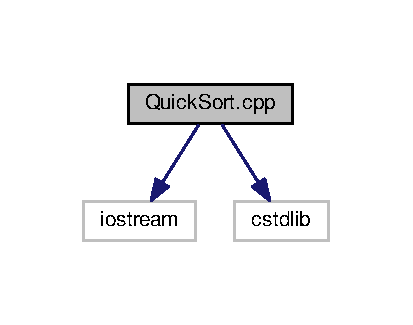
\includegraphics[width=198pt]{QuickSort_8cpp__incl}
\end{center}
\end{figure}
\subsection*{Functions}
\begin{DoxyCompactItemize}
\item 
void \hyperlink{QuickSort_8cpp_a4b9708d87be7a409eff20e5e7e8b43c8}{swap} (int $\ast$a, int $\ast$b)
\item 
int \hyperlink{QuickSort_8cpp_a672622cf23f5fe88cfa9bfe89d770b76}{Partition} (int a\mbox{[}$\,$\mbox{]}, int low, int high)
\item 
int \hyperlink{QuickSort_8cpp_aaf7e5bcba94f064d6f7a24e9a9cb74c4}{Random\+Pivot\+Partition} (int a\mbox{[}$\,$\mbox{]}, int low, int high)
\item 
int \hyperlink{QuickSort_8cpp_a091490bff9f594fbaec477e112f8938c}{Quick\+Sort} (int a\mbox{[}$\,$\mbox{]}, int low, int high)
\item 
int \hyperlink{QuickSort_8cpp_ae66f6b31b5ad750f1fe042a706a4e3d4}{main} ()
\end{DoxyCompactItemize}


\subsection{Function Documentation}
\index{Quick\+Sort.\+cpp@{Quick\+Sort.\+cpp}!main@{main}}
\index{main@{main}!Quick\+Sort.\+cpp@{Quick\+Sort.\+cpp}}
\subsubsection[{\texorpdfstring{main()}{main()}}]{\setlength{\rightskip}{0pt plus 5cm}int main (
\begin{DoxyParamCaption}
{}
\end{DoxyParamCaption}
)}\hypertarget{QuickSort_8cpp_ae66f6b31b5ad750f1fe042a706a4e3d4}{}\label{QuickSort_8cpp_ae66f6b31b5ad750f1fe042a706a4e3d4}

\begin{DoxyCode}
67 \{
68     \textcolor{keywordtype}{int} n, i;
69     cout<<\textcolor{stringliteral}{"\(\backslash\)nEnter the number of data element to be sorted: "};
70     cin>>n;
71  
72     \textcolor{keywordtype}{int} arr[n];
73     \textcolor{keywordflow}{for}(i = 0; i < n; i++)
74     \{
75         cout<<\textcolor{stringliteral}{"Enter element "}<<i+1<<\textcolor{stringliteral}{": "};
76         cin>>arr[i];
77     \}
78  
79     \hyperlink{QuickSort_8cpp_a091490bff9f594fbaec477e112f8938c}{QuickSort}(arr, 0, n-1);
80  
81     \textcolor{comment}{// Printing the sorted data.}
82     cout<<\textcolor{stringliteral}{"\(\backslash\)nSorted Data "};
83     \textcolor{keywordflow}{for} (i = 0; i < n; i++)
84             cout<<\textcolor{stringliteral}{"->"}<<arr[i];
85  
86     \textcolor{keywordflow}{return} 0;
87 \}\end{DoxyCode}


Here is the call graph for this function\+:
\nopagebreak
\begin{figure}[H]
\begin{center}
\leavevmode
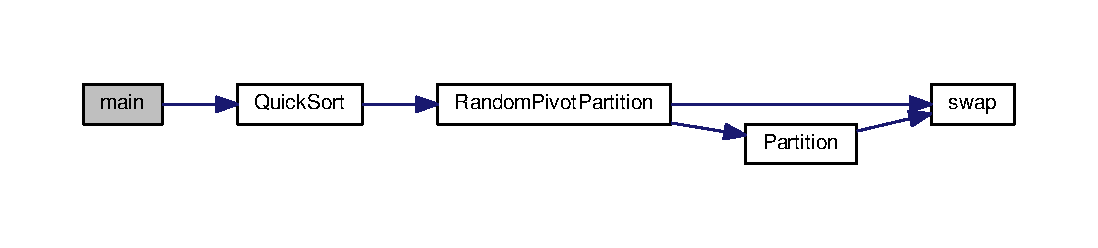
\includegraphics[width=350pt]{QuickSort_8cpp_ae66f6b31b5ad750f1fe042a706a4e3d4_cgraph}
\end{center}
\end{figure}


\index{Quick\+Sort.\+cpp@{Quick\+Sort.\+cpp}!Partition@{Partition}}
\index{Partition@{Partition}!Quick\+Sort.\+cpp@{Quick\+Sort.\+cpp}}
\subsubsection[{\texorpdfstring{Partition(int a[], int low, int high)}{Partition(int a[], int low, int high)}}]{\setlength{\rightskip}{0pt plus 5cm}int Partition (
\begin{DoxyParamCaption}
\item[{int}]{a\mbox{[}$\,$\mbox{]}, }
\item[{int}]{low, }
\item[{int}]{high}
\end{DoxyParamCaption}
)}\hypertarget{QuickSort_8cpp_a672622cf23f5fe88cfa9bfe89d770b76}{}\label{QuickSort_8cpp_a672622cf23f5fe88cfa9bfe89d770b76}

\begin{DoxyCode}
17 \{
18     \textcolor{keywordtype}{int} pivot, index, i;
19     index = low;
20     pivot = high;
21  
22     \textcolor{comment}{// Getting index of pivot.}
23     \textcolor{keywordflow}{for}(i=low; i < high; i++)
24     \{
25         \textcolor{keywordflow}{if}(a[i] < a[pivot])
26         \{
27             \hyperlink{QuickSort_8cpp_a4b9708d87be7a409eff20e5e7e8b43c8}{swap}(&a[i], &a[index]);
28             index++;
29         \}
30     \}
31     \textcolor{comment}{// Swapping value at high and at the index obtained.}
32     \hyperlink{QuickSort_8cpp_a4b9708d87be7a409eff20e5e7e8b43c8}{swap}(&a[pivot], &a[index]);
33  
34     \textcolor{keywordflow}{return} index;
35 \}
\end{DoxyCode}


Here is the call graph for this function\+:
\nopagebreak
\begin{figure}[H]
\begin{center}
\leavevmode
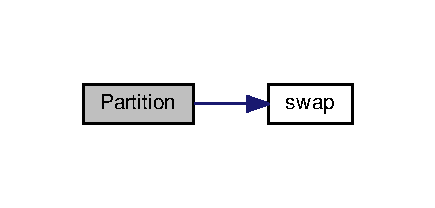
\includegraphics[width=209pt]{QuickSort_8cpp_a672622cf23f5fe88cfa9bfe89d770b76_cgraph}
\end{center}
\end{figure}


\index{Quick\+Sort.\+cpp@{Quick\+Sort.\+cpp}!Quick\+Sort@{Quick\+Sort}}
\index{Quick\+Sort@{Quick\+Sort}!Quick\+Sort.\+cpp@{Quick\+Sort.\+cpp}}
\subsubsection[{\texorpdfstring{Quick\+Sort(int a[], int low, int high)}{QuickSort(int a[], int low, int high)}}]{\setlength{\rightskip}{0pt plus 5cm}int Quick\+Sort (
\begin{DoxyParamCaption}
\item[{int}]{a\mbox{[}$\,$\mbox{]}, }
\item[{int}]{low, }
\item[{int}]{high}
\end{DoxyParamCaption}
)}\hypertarget{QuickSort_8cpp_a091490bff9f594fbaec477e112f8938c}{}\label{QuickSort_8cpp_a091490bff9f594fbaec477e112f8938c}

\begin{DoxyCode}
53 \{
54     \textcolor{keywordtype}{int} pindex;
55     \textcolor{keywordflow}{if}(low < high)
56     \{
57         \textcolor{comment}{// Partitioning array using randomized pivot.}
58         pindex = \hyperlink{QuickSort_8cpp_aaf7e5bcba94f064d6f7a24e9a9cb74c4}{RandomPivotPartition}(a, low, high);
59         \textcolor{comment}{// Recursively implementing QuickSort.}
60         \hyperlink{QuickSort_8cpp_a091490bff9f594fbaec477e112f8938c}{QuickSort}(a, low, pindex-1);
61         \hyperlink{QuickSort_8cpp_a091490bff9f594fbaec477e112f8938c}{QuickSort}(a, pindex+1, high);
62     \}
63     \textcolor{keywordflow}{return} 0;
64 \}
\end{DoxyCode}


Here is the call graph for this function\+:
\nopagebreak
\begin{figure}[H]
\begin{center}
\leavevmode
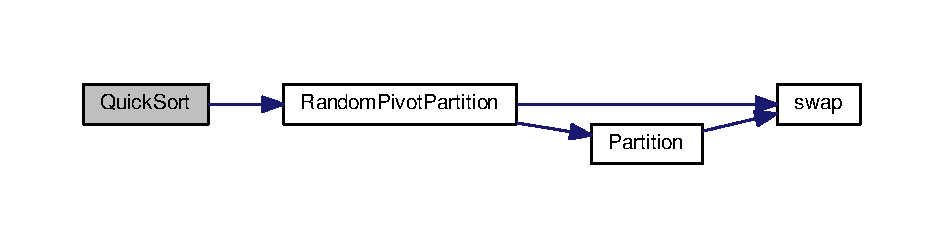
\includegraphics[width=350pt]{QuickSort_8cpp_a091490bff9f594fbaec477e112f8938c_cgraph}
\end{center}
\end{figure}


\index{Quick\+Sort.\+cpp@{Quick\+Sort.\+cpp}!Random\+Pivot\+Partition@{Random\+Pivot\+Partition}}
\index{Random\+Pivot\+Partition@{Random\+Pivot\+Partition}!Quick\+Sort.\+cpp@{Quick\+Sort.\+cpp}}
\subsubsection[{\texorpdfstring{Random\+Pivot\+Partition(int a[], int low, int high)}{RandomPivotPartition(int a[], int low, int high)}}]{\setlength{\rightskip}{0pt plus 5cm}int Random\+Pivot\+Partition (
\begin{DoxyParamCaption}
\item[{int}]{a\mbox{[}$\,$\mbox{]}, }
\item[{int}]{low, }
\item[{int}]{high}
\end{DoxyParamCaption}
)}\hypertarget{QuickSort_8cpp_aaf7e5bcba94f064d6f7a24e9a9cb74c4}{}\label{QuickSort_8cpp_aaf7e5bcba94f064d6f7a24e9a9cb74c4}

\begin{DoxyCode}
39 \{
40     \textcolor{keywordtype}{int} pvt, n, temp;
41     n = rand();
42     \textcolor{comment}{// Randomizing the pivot value in the given subpart of array.}
43     pvt = low + n%(high-low+1);
44  
45     \textcolor{comment}{// Swapping pvt value from high, so pvt value will be taken as pivot while partitioning.}
46     \hyperlink{QuickSort_8cpp_a4b9708d87be7a409eff20e5e7e8b43c8}{swap}(&a[high], &a[pvt]);
47  
48     \textcolor{keywordflow}{return} \hyperlink{QuickSort_8cpp_a672622cf23f5fe88cfa9bfe89d770b76}{Partition}(a, low, high);
49 \}
\end{DoxyCode}


Here is the call graph for this function\+:
\nopagebreak
\begin{figure}[H]
\begin{center}
\leavevmode
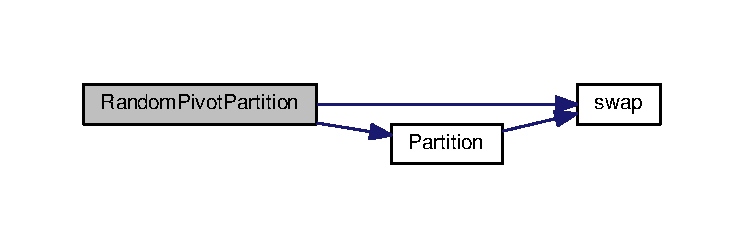
\includegraphics[width=350pt]{QuickSort_8cpp_aaf7e5bcba94f064d6f7a24e9a9cb74c4_cgraph}
\end{center}
\end{figure}


\index{Quick\+Sort.\+cpp@{Quick\+Sort.\+cpp}!swap@{swap}}
\index{swap@{swap}!Quick\+Sort.\+cpp@{Quick\+Sort.\+cpp}}
\subsubsection[{\texorpdfstring{swap(int $\ast$a, int $\ast$b)}{swap(int *a, int *b)}}]{\setlength{\rightskip}{0pt plus 5cm}void swap (
\begin{DoxyParamCaption}
\item[{int $\ast$}]{a, }
\item[{int $\ast$}]{b}
\end{DoxyParamCaption}
)}\hypertarget{QuickSort_8cpp_a4b9708d87be7a409eff20e5e7e8b43c8}{}\label{QuickSort_8cpp_a4b9708d87be7a409eff20e5e7e8b43c8}

\begin{DoxyCode}
8 \{
9     \textcolor{keywordtype}{int} temp; 
10     temp = *a;
11     *a = *b;
12     *b = temp;
13 \}
\end{DoxyCode}

%--- End generated contents ---

% Index
\backmatter
\newpage
\phantomsection
\clearemptydoublepage
\addcontentsline{toc}{chapter}{Index}
\printindex

\end{document}
